%% Wiki: [[2026.01.23 - Mathematics: Spectral Anonymity and Optimal Distinguishing Bounds for Random-Walk Delegation in (Possibly Directed) Overlays]]
\documentclass[11pt]{article}

% -------------------- layout and typography --------------------
\usepackage[margin=1in]{geometry}
\usepackage{microtype}
\setlength{\emergencystretch}{2.5em}

% -------------------- math --------------------
\usepackage{amsmath,amssymb,amsthm,mathtools}

% -------------------- tables and lists --------------------
\usepackage{booktabs}
\usepackage{graphicx}
\usepackage{tabularx}
\usepackage{array}
\usepackage{enumitem}

% -------------------- plots (optional, self-contained) --------------------
\usepackage{pgfplots}
\pgfplotsset{compat=1.18}

% -------------------- hyperlinks and references --------------------
\usepackage[hidelinks]{hyperref}
\usepackage[nameinlink,noabbrev]{cleveref}

% -------------------- theorem environments --------------------
\newtheorem{theorem}{Theorem}[section]
\newtheorem{lemma}[theorem]{Lemma}
\newtheorem{corollary}[theorem]{Corollary}
\newtheorem{definition}[theorem]{Definition}
\newtheorem{proposition}[theorem]{Proposition}
\newtheorem{remark}[theorem]{Remark}

% -------------------- convenient columns --------------------
\newcolumntype{Y}{>{\raggedright\arraybackslash}X}
\newcolumntype{L}[1]{>{\raggedright\arraybackslash}p{#1}}

% -------------------- macros --------------------
\newcommand{\TV}{\mathrm{TV}}
\newcommand{\KL}{\mathrm{KL}}
\newcommand{\E}{\mathbb{E}}
\newcommand{\Prb}{\mathbb{P}}
\newcommand{\Unif}{\mathrm{Unif}}
\newcommand{\cD}{\mathcal{D}}
\newcommand{\PiM}{\Pi}

\title{Spectral Anonymity and Optimal Distinguishing Bounds\\for Random-Walk Delegation in (Possibly Directed) Overlays}
\author{}
\date{January 23, 2026}

\begin{document}
\maketitle

\noindent\textbf{Canonical wiki page:} \texttt{[[2026.01.23 - Mathematics: Spectral Anonymity and Optimal Distinguishing Bounds for Random-Walk Delegation in (Possibly Directed) Overlays]]}\\


\begin{abstract}
A common anonymity pattern in overlay routing is \emph{random-walk delegation}:
an initiator performs a short random walk to pick a \emph{delegate} and asks the
delegate to execute a normal lookup. We develop a compact, proof-oriented
anonymity theory for delegate-only observers.

Our organizing lens is structural: under a stationary initiator prior, the
posterior distribution of the initiator given the observed delegate is exactly
the $t$-step law of the \emph{time-reversed} chain started at that delegate.
This reduction turns delegate-only anonymity questions into standard mixing
questions (including on directed/nonreversible overlays). We derive sharp
distinguishing bounds in total variation distance and give leakage certificates:
a conservative $\sigma^t$ bound via $\ell_2(\pi)$ contraction and an \emph{exact}
expected $\chi^2$ (R\'enyi-2) leakage identity in terms of the \emph{full}
singular spectrum of the discriminant operator.

For space, this manuscript includes a \emph{reconstruction specification} and a
small set of \emph{sanity-check tables} rather than embedding full code and logs.
A complete artifact bundle (scripts, raw outputs, and plotting) is available as
supplementary material.
\end{abstract}

\section{Introduction}\label{sec:intro}
Many privacy-preserving overlay protocols hide who initiated a lookup by
forwarding the request through one or more intermediate relays, often selected
by random walks. Random-walk selection appears across anonymous DHT lookup and
relay-discovery systems (e.g., Octopus~\cite{octopus}, ShadowWalker~\cite{shadowwalker}, NISAN~\cite{nisan}) and in early
foundational models such as Crowds.

\paragraph{Primitive (fixed-length delegation).}
An initiator $S$ runs a length-$t$ random walk on the overlay to sample a
delegate $D$, then asks $D$ to execute a standard lookup. Our core threat model
assumes the adversary learns only the delegate identity $D$ for a single
delegation. (We briefly discuss ``first-hit'' compromise observations in
\cref{sec:compromise}.)

\paragraph{What is new here.}
The posterior-as-time-reversal identity is elementary, but it is \emph{useful as
a reduction}: it makes the anonymity analysis of delegation \emph{exactly} a
mixing analysis problem, including for directed/nonreversible overlays. The
main technical contributions are the resulting optimal distinguishability bounds
and computable leakage certificates for directed chains, including a
full-spectrum (not only $\sigma_2$) identity.

\paragraph{Main results.}
Let $P$ be the walk kernel on node set $V$ with stationary $\pi$ and let $P^\star$
be its time reversal.
\begin{itemize}[leftmargin=1.2em]
\item \textbf{Posterior structure (tool).} Under $S\sim\pi$, the posterior is a
reversed walk: $\Prb[S=\cdot\mid D=d]=(P^\star)^t(d,\cdot)$ (\cref{thm:posterior}).
\item \textbf{Optimal tests.} Any test distinguishing two candidate initiators
from the delegate identity has optimal advantage equal to total variation
distance between their delegate laws (\cref{cor:opt-test}).
\item \textbf{Spectral certificates, including full spectrum.} Let
$\cD=\Pi^{1/2}P\Pi^{-1/2}$ be the discriminant operator with singular values
$1=\sigma_1\ge\sigma_2\ge\cdots\ge\sigma_n$. We give (i) a conservative bound
$\E[\chi^2(\Pr[S=\cdot\mid D]\|\pi)]\le\sigma_2^{2t}$ and (ii) an exact identity
$\E[\chi^2(\Pr[S=\cdot\mid D]\|\pi)]=\sum_{i=2}^n\sigma_i^{2t}$
(\cref{thm:chi2-exact}).
\item \textbf{Perfect delegation.} Stopping at a strong stationary time yields a
delegate distributed exactly as $\pi$ and independent of $S$ (perfect anonymity
against delegate-only observers; \cref{sec:sst}).
\item \textbf{Non-normal cautionary example.} Directed de Bruijn overlays mix in
finite time yet can have $\sigma_2\approx 1$, making $\sigma_2^t$ bounds vacuous
(\cref{sec:debruijn}).
\end{itemize}

\paragraph{Limitations (explicit).}
This paper deliberately targets \emph{delegate-only} observation and a
\emph{fixed} kernel $P$. We do \emph{not} model global passive traffic analysis
(timing/volume correlation, batching, packet sizes), active/adaptive adversaries
(e.g., dropping/biasing forwarding, Sybil/route-capture), or multi-point
observation beyond the delegate identity. We also do not model churn and other
time-variation in the overlay itself: if the kernel changes over time
($P_t$), the certificates in this paper should be read as snapshot guarantees
and can degrade toward a noise floor as churn ``resets'' the mixing clock.

\paragraph{Artifacts and reconstruction.}
To keep the manuscript compact, we include only a reconstruction specification
and sanity-check tables. Full scripts, raw outputs, and plotting are available
as supplementary material.


\section{How to read and verify (LLM-friendly)}\label{sec:howtoread}
This paper is organized around two ``hinge'' facts that let you translate
delegation anonymity questions into standard Markov-chain objects.

\begin{itemize}[leftmargin=1.2em]
\item \textbf{Hinge 1 (posterior as time reversal).} Given a delegate $D=d$ under
a stationary initiator prior, the posterior on the initiator is \emph{exactly}
a reversed walk started at $d$ (\cref{thm:posterior}). You can treat this as a
reduction: any bound on how fast a chain ``forgets its start'' can be imported
as an anonymity statement for delegation.
\item \textbf{Hinge 2 (expected $\chi^2$ leakage as a spectrum).} The expected
R\'enyi-2 leakage has an \emph{exact} formula in terms of the singular spectrum
of the discriminant operator (\cref{thm:chi2-exact}). This supplies a computable
certificate that remains informative for directed/non-normal overlays where the
single-number $\sigma_2$ bound can be misleading.
\end{itemize}

\paragraph{Fast verification path.}
A quick referee-style check is:
(i) verify \cref{thm:posterior} by Bayes + time reversal;
(ii) verify \cref{thm:chi2-exact} by rewriting expected collision probability as a Frobenius norm;
(iii) reproduce \cref{tab:families,tab:firsthit-sweep} from the reconstruction spec in \cref{sec:reconstruct}.
Full scripts and raw outputs are available as supplementary material.

\section{Related work and context}\label{sec:related}
Random-walk-based relay selection has a long history in anonymity systems, from
early models such as \emph{Crowds} to anonymous lookup schemes for structured
overlays. Our focus is deliberately narrow: we isolate the \emph{delegation}
primitive and ask what can be inferred from the \emph{delegate identity alone}.
This lens complements system papers that treat richer adversaries (timing,
volume, route-capture, Sybils) by providing sharp and composable bounds for the
delegate-only component.

For concrete systems that instantiate random-walk relay selection and/or anonymous lookup in structured overlays, see ShadowWalker~\cite{shadowwalker} (random-walk-based peer-to-peer anonymity over structured topologies), NISAN~\cite{nisan} (DHT-based network information service for anonymization networks), and Octopus~\cite{octopus} (secure and anonymous DHT lookup).

On the Markov-chain side, we use standard notions from mixing theory---total
variation and separation distance, time reversal, and strong stationary times.
Background can be found in Levin--Peres--Wilmer \cite{lpw} and in the original
strong-stationary-time work of Aldous--Diaconis \cite{aldousdiaconis}; see also
Fill \cite{fill} for related perspectives. On the systems side, our results
provide a principled way to interpret (and sometimes refute) common heuristics
that ``a spectral gap guarantees privacy,'' especially for directed overlays.
We also relate to work on adding query privacy to robust DHTs \cite{backes} and
to classic relay-anonymity models \cite{reiterrubin}.

\section{Model and definitions}\label{sec:model}
Let $V$ be a finite set of nodes, $|V|=n$. Let $P$ be a (row-stochastic) Markov
kernel on $V$ with stationary distribution $\pi$ satisfying $\pi(x)>0$ for all
$x$. We allow $P$ to be directed and nonreversible.

\paragraph{Delegation experiment.}
Sample an initiator $S\sim \pi$. Starting from $S$, run the chain for $t$ steps
and output the endpoint $D$ (the delegate):
\[
\Prb[D=d\mid S=s] = P^t(s,d).
\]

\paragraph{Time reversal.}
Define the time-reversed kernel $P^\star$ by
\begin{equation}\label{eq:rev}
\pi(x)P(x,y)=\pi(y)P^\star(y,x)\qquad(\forall x,y\in V),
\end{equation}
so $P^\star(y,x)=\pi(x)P(x,y)/\pi(y)$.

\paragraph{Distances and leakage.}
For distributions $\mu,\nu$ on $V$,
\[
\TV(\mu,\nu)=\tfrac12\sum_{x\in V}|\mu(x)-\nu(x)|.
\]
The Pearson chi-squared divergence is
\[
\chi^2(\mu\|\pi)=\sum_{x\in V}\frac{(\mu(x)-\pi(x))^2}{\pi(x)}
=\sum_{x\in V}\frac{\mu(x)^2}{\pi(x)}-1.
\]
We use conditional min-entropy
$H_\infty(S\mid D)= -\log \sum_d \Prb[D=d]\max_s \Prb[S=s\mid D=d]$.

\section{Posterior structure and optimal tests}\label{sec:posterior}
\begin{theorem}[Posterior equals reversed walk]\label{thm:posterior}
Assume $S\sim \pi$ and $D$ is obtained by a length-$t$ walk from $S$ using $P$.
Then for every $d\in V$,
\[
\Prb[S=s\mid D=d] = (P^\star)^t(d,s)\qquad(\forall s\in V).
\]
\end{theorem}
\begin{proof}
Bayes' rule gives
$\Prb[S=s\mid D=d]=\frac{P^t(s,d)\pi(s)}{\sum_u P^t(u,d)\pi(u)}$.
Stationarity implies $\sum_u \pi(u)P^t(u,d)=\pi(d)$, hence
$\Prb[S=s\mid D=d]=\pi(s)P^t(s,d)/\pi(d)$. Applying \eqref{eq:rev} $t$ times
yields $\pi(s)P^t(s,d)=\pi(d)(P^\star)^t(d,s)$.
\end{proof}

\begin{proposition}[Time-varying kernels]\label{prop:inhom}
The posterior-as-reversal lens extends verbatim to time-inhomogeneous walks.
Let $P_1,\dots,P_t$ be a sequence of Markov kernels that share a stationary
distribution $\pi$ (i.e., $\pi P_i=\pi$ for all $i$). Sample $S\sim\pi$ and run
the inhomogeneous chain $X_0=S$, $X_{i}=X_{i-1}P_i$, and output $D=X_t$.
Then, for every $d\in V$,
\[
\Prb[S=s\mid D=d] \;=\; (P_t^\star P_{t-1}^\star\cdots P_1^\star)(d,s),
\]
where $P_i^\star$ is the time reversal of $P_i$ with respect to $\pi$.
\end{proposition}

\begin{proof}
By Bayes' rule,
$\Prb[S=s\mid D=d]=\pi(s)(P_1\cdots P_t)(s,d)/\pi(d)$, using $\Prb[D=d]=\pi(d)$.
Applying the single-step reversal identity $\pi(x)P_i(x,y)=\pi(y)P_i^\star(y,x)$
along the product yields $(P_t^\star\cdots P_1^\star)(d,s)$.
\end{proof}

\begin{remark}[Churn as perturbation]
If churn changes the kernel over time but approximately preserves a common
stationary distribution, \cref{prop:inhom} shows that the anonymity analysis is
still an exact reversal of the \emph{actual} time-varying walk.
If stationarity itself drifts, the snapshot results in this paper should be
interpreted as local guarantees that can degrade toward a noise floor.
\end{remark}



\begin{remark}[Framing]\label{rem:lens}
\cref{thm:posterior} is a one-line calculation, but it is the key \emph{lens} of
this paper: it converts delegate-only anonymity analysis into standard mixing
analysis on the reversed chain, including for directed/nonreversible overlays.
\end{remark}

\begin{corollary}[Optimal test]\label{cor:opt-test}
For any two candidates $s_0,s_1\in V$ and any (possibly randomized) test
$\phi:V\to\{0,1\}$ based only on $D$,
\[
\max_{\phi}\Big|\Prb[\phi(D)=1\mid S=s_0]-\Prb[\phi(D)=1\mid S=s_1]\Big|
= \TV\!\big(P^t(s_0,\cdot),\,P^t(s_1,\cdot)\big).
\]
\end{corollary}
\begin{proof}
Classical characterization of total variation distance as optimal distinguishing
advantage between two distributions.
\end{proof}

\section{Spectral anonymity bounds}\label{sec:spectral}
For reversible chains, mixing is governed by eigenvalues; for directed chains,
singular values of the \emph{discriminant} operator play the analogous role.

\begin{definition}[Discriminant operator]\label{def:disc}
Let $\PiM=\mathrm{diag}(\pi)$. Define
\[
\cD \;=\; \PiM^{1/2} P \PiM^{-1/2}.
\]
Let $1=\sigma_1\ge\sigma_2\ge\cdots\ge\sigma_n\ge 0$ be its singular values.
\end{definition}

\begin{theorem}[Exact expected chi-squared leakage]\label{thm:chi2-exact}
Under the stationary prior, let $\mu_d(\cdot)=\Prb[S=\cdot\mid D=d]$. Then
\[
\E_{D\sim \pi}\!\left[\chi^2(\mu_D\|\pi)\right] \;=\;
\sum_{i=2}^n \sigma_i^{2t}.
\]
\end{theorem}
\begin{proof}[Proof sketch]
Let $M=\PiM^{1/2}P^t\PiM^{-1/2}=\cD^t$. One can rewrite
$\E_{D\sim\pi}\left[\sum_s \mu_D(s)^2/\pi(s)\right]$ as the Frobenius norm
$\|M\|_F^2$, which equals the sum of squared singular values of $M$, namely
$\sum_i \sigma_i^{2t}$. Subtract the $i=1$ term.
\end{proof}

\begin{corollary}[Conservative $\sigma_2$ certificate]\label{cor:sigma2}
Since $\sum_{i=2}^n \sigma_i^{2t}\le (n-1)\sigma_2^{2t}$,
\[
\E_{D\sim\pi}\!\left[\chi^2(\mu_D\|\pi)\right]\le (n-1)\sigma_2^{2t},
\qquad
\E[\TV(\mu_D,\pi)] \le \tfrac12\sqrt{(n-1)}\,\sigma_2^{t}.
\]
\end{corollary}

\paragraph{Why full spectrum matters.}
For non-normal directed chains, $\sigma_2$ can be close to 1 even when the chain
mixes quickly (see \cref{sec:debruijn}); \cref{thm:chi2-exact} can remain sharp
because most singular values may be small or zero.

\section{Perfect delegation via strong stationary times}\label{sec:sst}
\begin{definition}[Strong stationary time]
A stopping time $T$ is a \emph{strong stationary time} if $X_T\sim\pi$ and
$X_T$ is independent of $T$.
\end{definition}

\begin{theorem}[Perfect anonymity against delegate-only observers]
If delegation outputs $D=X_T$ for a strong stationary time $T$, then $D\sim\pi$
and $D$ is independent of $S$. Hence $\Prb[S=s\mid D=d]=\pi(s)$ for all $s,d$.
\end{theorem}
\begin{proof}
Immediate from the definition of strong stationary time and independence.
\end{proof}

\section{Repeated lookups: tensorization}\label{sec:repeated}
Suppose the same initiator performs $k$ independent delegations, producing
delegates $D_1,\dots,D_k$.

\begin{proposition}[Posterior tensorizes]\label{prop:tensor}
Under a stationary prior and conditional independence of walks,
\[
\Prb[S=s\mid D_1=d_1,\dots,D_k=d_k]
\;\propto\; \pi(s)\prod_{j=1}^k P^t(s,d_j).
\]
\end{proposition}
\begin{proof}
Bayes' rule and conditional independence:
$\Prb[D_1=d_1,\dots,D_k=d_k\mid S=s]=\prod_j P^t(s,d_j)$.
\end{proof}

\paragraph{Amplification (interpretation).}
The optimal distinguishing advantage between two candidates from the vector
$(D_1,\dots,D_k)$ is the total variation distance between the corresponding
product laws $P^t(s_i,\cdot)^{\otimes k}$. For large $n$, exact computation of
product-TV or Chernoff information is typically impractical; in practice, one
can upper-bound amplification using additive divergences (e.g., KL) or use the
single-delegation certificates as conservative proxies.


\section{Randomized walk length and hopcount leakage}\label{sec:randlen}
Some systems randomize the walk length (hopcount) to reduce latency or to
complicate inference. Let $T$ be an integer-valued random walk length, sampled
independently of the initiator and of the walk transitions, and let the delegate
be $D=X_T$.

\begin{proposition}[Posterior under randomized length]\label{prop:randlen}
Assume $S\sim\pi$ and $T\perp S$. Then:
\begin{enumerate}[leftmargin=1.6em]
\item If the adversary observes both $(D,T)=(d,t)$, then
$\Prb[S=\cdot\mid D=d,T=t]=(P^\star)^t(d,\cdot)$.
\item If the adversary observes only $D=d$, then the posterior is a mixture of
reversed walks:
\[
\Prb[S=s\mid D=d] \;=\; \sum_{t\ge 0} \Prb[T=t]\,(P^\star)^t(d,s).
\]
\end{enumerate}
\end{proposition}

\begin{proof}
For (1), condition on $T=t$ and apply \cref{thm:posterior}. For (2),
$\Prb[S=s\mid D=d]\propto \pi(s)\sum_t \Prb[T=t]P^t(s,d)$ and the denominator
equals $\pi(d)$ by stationarity; rewrite each term using time reversal.
\end{proof}

\paragraph{Design guidance.}
Randomizing length only helps if it prevents the adversary from conditioning on
short walks. In particular, if $T$ has nontrivial probability on small values,
then the mixture in \cref{prop:randlen} retains a ``short-walk'' component that
can dominate leakage. A practical pattern is \emph{burn-in plus a tail}:
choose a minimum $t_{\min}$ that already meets a leakage target, and then add a
random tail (e.g., geometric) whose realization is hidden by padding or batching.
Full analyses for specific hopcount distributions are included in the artifact
bundle.

\section{Compromised nodes and ``early observation''}\label{sec:compromise}
A common deviation from the pure delegate-only model is that an adversary who
compromises a set $C\subseteq V$ may learn the first time a walk hits $C$ (and
possibly which compromised node was hit first). Even without timing, this
``first-hit'' observation can leak information beyond the delegate identity.

We treat a simple time-hidden model in \cref{sec:experiments} as a robustness
check: the adversary learns only the identity of the first compromised node hit
within a fixed horizon, if any.

\section{Exact mixing on directed de Bruijn overlays}\label{sec:debruijn}
The directed de Bruijn graph $B(k,m)$ has $n=k^m$ nodes labeled by length-$m$
strings. A move shifts left and appends a fresh symbol. The non-lazy walk mixes
\emph{exactly} in $m$ steps (the last $m$ appended symbols determine the state),
yet the walk is highly non-normal.

\begin{remark}[Finite-time mixing vs $\sigma_2$]
On the non-lazy de Bruijn walk, the usual $\sigma_2^t$ intuition can mislead:
the chain reaches stationarity in $m$ steps, but singular-value bounds can be
vacuous if $\sigma_2\approx 1$. Full-spectrum leakage identities are therefore
a better diagnostic on directed overlays.
\end{remark}

\paragraph{Deterministic suffix leakage.}
In the non-lazy de Bruijn walk, the delegate reveals a deterministic suffix of
the initiator (the last $m-t$ symbols) because shifting discards a prefix. This
illustrates that ``mixing in distribution'' and ``hiding structured attributes''
can diverge unless the threat model and protocol details are aligned.


\section{Practical guidance: which bound to use}\label{sec:guidance}
This section summarizes how to turn the theory into ``engineering numbers'' and
how to match a leakage question to a certificate.

\begin{table}[h]
\centering
\small
\setlength{\tabcolsep}{4pt}
\renewcommand{\arraystretch}{1.15}
\begin{tabularx}{\linewidth}{>{\raggedright\arraybackslash}p{0.24\linewidth}>{\raggedright\arraybackslash}p{0.27\linewidth}>{\raggedright\arraybackslash}X}
\toprule
Goal & Suggested quantity & How to estimate / interpret \\
\midrule
Best test between two candidate initiators
& $\TV(P^t(s_0,\cdot),P^t(s_1,\cdot))$
& Exact optimal advantage (\cref{cor:opt-test}); estimate by Monte Carlo when $n$ is large. \\
Average ``distance from uniform'' of the posterior
& $\E[\chi^2(\Pr[S=\cdot\mid D]\|\pi)]$
& Exact identity $\sum_{i\ge 2}\sigma_i^{2t}$ (\cref{thm:chi2-exact}); approximate using a few leading singular values. \\
Conservative quick bound on average leakage
& $\sigma_2^{2t}$
& Easy to compute but can be loose on non-normal digraphs; use as a pessimistic upper bound (\cref{cor:sigma2}). \\
Worst-case spikes
& separation distance
& Controls the maximum posterior ratio; estimate via $\min_x P^t(s,x)/\pi(x)$ (simulation or sparse powering). \\
\bottomrule
\end{tabularx}
\caption{Certificate menu for delegate-only leakage questions.}
\label{tab:menu}
\end{table}

\paragraph{Threat-model ladder (what the adversary observes).}
The delegate-only model is the baseline. Conditioning on additional side
information typically strengthens the adversary; the posterior lens remains the
right way to incorporate it:
\begin{itemize}[leftmargin=1.2em]
\item \textbf{Delegate only:} observe $D$; posterior is a reversed walk (\cref{thm:posterior}).
\item \textbf{Delegate + hopcount:} observe $(D,T)$; posterior is $(P^\star)^T(d,\cdot)$ (\cref{prop:randlen}).
\item \textbf{First-hit compromise:} observe first compromised node hit (possibly time-hidden); see \cref{sec:compromise}.
\item \textbf{Global timing/volume, route capture, Sybils:} out of scope (see \cref{sec:intro}).
\end{itemize}

\subsection*{Design recommendations (turning bounds into protocol knobs)}
This subsection translates the theory into actionable choices of walk kernel,
walk length, and operational mitigations.

\paragraph{R1. Pick an attacker metric and set a numeric target.}
If the adversary is comparing two candidates, total variation is the right unit:
target $\varepsilon$ and choose parameters so that
$\TV(P^t(s_0,\cdot),P^t(s_1,\cdot))\le \varepsilon$ for the relevant pairs
(\cref{cor:opt-test}). If you want ``posterior close to prior on average,''
target $\E[\chi^2(\Pr[S=\cdot\mid D]\|\pi)]\le \delta$ or
$\E[\TV(\Pr[S=\cdot\mid D],\pi)]\le \varepsilon$.

\paragraph{R2. Use the full-spectrum certificate when $P$ is directed.}
On directed/non-normal overlays, $\sigma_2$ can dramatically mis-predict privacy
(\cref{sec:debruijn}). When possible, estimate the leading singular values of the
discriminant operator and choose the smallest $t$ such that
$\sum_{i\ge 2}\sigma_i^{2t}\le \delta$ (\cref{thm:chi2-exact}). If you only have
$\sigma_2$, treat $\sigma_2^{2t}$ as a conservative upper bound (\cref{cor:sigma2}),
not a calibrated estimate.

\paragraph{R3. Fix structural leakage in the kernel before tuning $t$.}
A longer walk does not help if the kernel deterministically preserves identifying
structure (e.g., a shift-like update on labels, \cref{sec:debruijn}). Low-cost
kernel modifications that usually improve privacy are:
(i) add laziness $P_{\text{lazy}}=\alpha I+(1-\alpha)P$,
(ii) add a small teleport mixture $\alpha \mathbf{1}\pi^\top+(1-\alpha)P$,
and (iii) prefer Eulerian/near-regular overlays so $\pi$ is simple.

\paragraph{R4. Make repeated queries a first-class design dimension.}
If an observer can link $k$ delegations to the same initiator, posteriors
multiply (\cref{sec:repeated}) and leakage can amplify. Either increase $t$ to
meet targets at the session level, or break linkage via key rotation/pseudonyms,
rate limits, batching, or enforced cool-down windows.

\paragraph{R5. If you randomize hopcount, hide it and include burn-in.}
Revealed hopcount strengthens the adversary: conditioning on $T$ produces a
sharper posterior (\cref{sec:randlen}). If you randomize length, keep hopcount
hidden and use a \emph{burn-in plus tail} distribution (e.g., $T=t_0+G$ with
geometric $G$) so every delegation mixes at least $t_0$ steps while the tail
obscures exact length.

\paragraph{R6. Treat churn as a noise floor; re-estimate periodically.}
The clean certificates assume a fixed $P$. With churn, the operational kernel is
time-varying. If instantaneous kernels share $\pi$, the reversal lens extends to
inhomogeneous products (\cref{prop:inhom}); otherwise churn perturbs both $P$ and
$\pi$, typically imposing a residual leakage floor. In practice: add modest
laziness/teleportation, avoid brittle deterministic routing steps, and
periodically recompute certificates on current snapshots.

\paragraph{R7. Prefer strong stationary times when feasible.}
An SST-based stop yields perfect delegate-only anonymity (\cref{sec:sst}). If you
can implement an exact or approximate SST, it dominates fixed-$t$ tuning.

\paragraph{Implementation recipe.}
(1) choose the threat-model rung; (2) choose a leakage unit (TV or expected
$\chi^2$) and a numeric target; (3) choose a privacy-friendly kernel; (4) estimate
a certificate (prefer full-spectrum); (5) pick the smallest $t$ meeting the
target; (6) revisit if linkage or churn changes your regime.



\subsection*{Design recommendations (expanded: protocol knobs, calibration, and pitfalls)}
The menu in \cref{tab:menu} tells you \emph{which} certificate matches a question. This section tells you
\emph{what to do} with those numbers.

\paragraph{Knobs-to-effects.}
\begin{table}[h]
\centering
\small
\setlength{\tabcolsep}{4pt}
\renewcommand{\arraystretch}{1.18}
\begin{tabularx}{\linewidth}{L{0.20\linewidth}Y Y}
\toprule
Knob & What it buys (privacy) & Cost / how to validate \\
\midrule
Increase walk length $t$ &
Reduces delegate-only leakage as the reversed walk mixes; the sharpest statement is the optimal TV test (\,\cref{cor:opt-test}\,) and the expected $\chi^2$ identity (\,\cref{thm:chi2-exact}\,). &
Latency, bandwidth, and exposure to compromise during the walk. Validate with pairwise TV on the cohort you care about, and/or $\sum_{i\ge2}\sigma_i^{2t}$. \\

Add laziness / self-loops &
Damps periodicity, smooths worst-case spikes, and makes metrics more stable under mild nonstationarity. &
Adds hops. Validate by re-estimating $t_{0.1}$ and checking separation distance. \\

Small teleport mixture to $\pi$ (or an approximate directory) &
Creates a robust ``mixing floor'' even under churn; combats deterministic structure and non-normal transients. &
Requires a sampling primitive approximating $\pi$; can be amortized via cached samples. Validate by checking that the teleport mass dominates the minimum-probability ratio. \\

Hide hopcount (and use burn-in + tail) &
Prevents conditioning on $T$; the posterior becomes a mixture of reversed walks (\,\cref{prop:randlen}\,). &
Must avoid side channels that leak length (timeouts, packet counts, retransmits). Validate by evaluating both (D-only) and (D,T) attack models. \\

Break linkability across queries &
Prevents tensorization amplification (\,\cref{sec:repeated}\,); makes ``per-query'' tuning meaningful. &
Requires protocol-level unlinkability (ephemeral IDs, batching, rate limits). Validate by enumerating what an adversary can realistically link. \\

SST / near-SST stopping &
If exact SST is implementable, yields perfect delegate-only anonymity (\,\cref{sec:sst}\,) and makes stopping adaptive. &
Harder to implement; may require additional randomness or certificates. Validate by checking that delegates are empirically $\pi$-distributed for many starts. \\
\bottomrule
\end{tabularx}
\caption{Protocol knobs and what the mathematics predicts they do.}
\label{tab:knobs}
\end{table}

\paragraph{Calibration patterns (how to pick $t$).}
Two simple patterns cover many deployments.
\begin{itemize}[leftmargin=1.2em]
\item \textbf{Pairwise indistinguishability target (TV).} Identify the pairs of starts that matter
(e.g., any two initiators in the same ASN/rack/region, or any two users in a cohort). Choose $t$ so that
$\max_{(s_0,s_1)\in\mathcal{P}} \TV(P^t(s_0,\cdot),P^t(s_1,\cdot)) \le \varepsilon$.
This aligns directly with optimal tests (\,\cref{cor:opt-test}\,). At large $n$, estimate each TV
by sampling delegates from each start and using a plug-in TV estimate or a held-out classifier.
\item \textbf{Average posterior drift target (expected $\chi^2$).} Choose $\delta$ and pick the smallest $t$ with
$\sum_{i\ge2}\sigma_i^{2t}\le\delta$ (\,\cref{thm:chi2-exact}\,). When computing the full spectrum is too costly,
estimate a few leading $\sigma_i$ and bound the remainder by $(n-r)\sigma_{r+1}^{2t}$.
\end{itemize}

\paragraph{Estimating certificates when $n$ is huge.}
The theory is finite-$n$, but estimation is often sublinear. Useful options:
\begin{itemize}[leftmargin=1.2em]
\item \textbf{Sampling-based TV/separation.} If you can run many delegations from a start $s$,
estimate $P^t(s,\cdot)$ empirically and compute TV/separation against a baseline. This is the most
system-faithful approach.
\item \textbf{Randomized SVD for top singular values.} On sparse kernels, randomized methods estimate the top
$\sigma_i$ of the discriminant operator $\cD$ using only matrix--vector products.
\item \textbf{Stochastic trace estimation for $\sum\sigma_i^{2t}$.} Since
$\sum_{i}\sigma_i^{2t}=\|\cD^t\|_F^2=\mathrm{tr}((\cD^\top\cD)^t)$,
one can estimate $\mathrm{tr}(A^t)$ for $A=\cD^\top\cD$ with Hutchinson estimators
($z^\top A^t z$ for random Rademacher $z$) using repeated sparse multiplies by $A$.
This targets the expected-$\chi^2$ certificate directly.
\end{itemize}

\paragraph{Common pitfalls.}
\begin{itemize}[leftmargin=1.2em]
\item \textbf{Mixing-to-$\pi$ from one start is not enough.} You want indistinguishability between \emph{different} starts.
Check pairwise TV (or a max-over-cohort) rather than only $\TV(P^t(s,\cdot),\pi)$.
\item \textbf{Non-normality breaks ``$\sigma_2$ intuition.''} On directed overlays treat $\sigma_2$ as a conservative bound,
not as a calibrated prediction (\,\cref{sec:debruijn}\,).
\item \textbf{Side channels can reintroduce hopcount.} If length can be inferred from timing, packet counts, or failure behavior,
then the relevant posterior is conditioned on $T$ (\,\cref{sec:randlen}\,).
\item \textbf{Churn can dominate.} If the overlay changes substantially over the delegation window,
certificates computed on stale snapshots may be irrelevant. Treat churn as a background ``leakage floor'' and
re-estimate on rolling snapshots (\,\cref{sec:intro}\,).
\end{itemize}

\paragraph{Speculative but plausible: continuous privacy control loops.}
Because building evaluators is now cheap, it is plausible to operationalize the mathematics as a control loop:
snapshot the overlay into a sparse kernel $P$; estimate certificates for a grid of $t$; pick the smallest $t$
meeting policy; and alert when churn or compromise pushes measured leakage above threshold.
Even if estimates are noisy, this replaces folklore with measurable guardrails.


\section{Sanity-check experiments (compact)}\label{sec:experiments}
We include two small tables to make reconstruction easy and to anchor the scale
of the bounds. Full experiments, additional sweeps, and plotting are available as
supplementary material.

\paragraph{Family comparison at $n=1024$.}
We compare 1/2-lazy random-walk mixing behavior on several $n=1024$-node regular
graph families, including a simple Chord-like ring-with-fingers digraph.
For each family we report the measured time $t_{0.1}$ to reach
$\TV(P^t(0,\cdot),\pi)\le 0.1$, along with separation distance at that time.
We also report a conservative $\sigma$-based prediction obtained by solving
$\tfrac12\sqrt{n}\,\sigma^t\le 0.1$ (using $\ell_2\!\to\!\ell_1$).

\begin{table}[h]
\centering
\small
\setlength{\tabcolsep}{4pt}
\begin{tabular}{lrrrrrr}
\toprule
Family & $d$ & $\sigma$ & measured $t_{0.1}$ & TV@ $t_{0.1}$ & Sep@ $t_{0.1}$ & pred.\ $t_{0.1}$ \\
\midrule
Cycle $C_n$ & 2 & 0.999991 & 196657 & 0.1000 & 0.3129 & 539201 \\
2D torus ($32\times 32$) & 4 & 0.995196 & 438 & 0.1000 & 0.4264 & 1054 \\
Hypercube $Q_{10}$ & 10 & 0.900000 & 25 & 0.0904 & 0.5634 & 49 \\
Chord ring+fingers & 10 & 0.900000 & 18 & 0.0989 & 0.7633 & 49 \\
Random 8-regular & 8 & 0.826246 & 15 & 0.0905 & 0.3325 & 27 \\
Directed de Bruijn $B(2,10)$ & 2 & 0.988831 & 24 & 0.0769 & 0.1537 & 452 \\
\bottomrule
\end{tabular}
\caption{Sanity-check family comparison ($n=1024$, 1/2-lazy walks, fixed start $0$).}
\label{tab:families}
\end{table}

\paragraph{Visualization: smooth vs.\ cliff mixing.}
To make the non-normal cautionary point visual, \cref{fig:tv-cliff} plots
$\TV(P^t(0,\cdot),\pi)$ for a 1/2-lazy cycle on $n=1024$ (slow, smooth decay)
against the \emph{non-lazy} directed de Bruijn walk on $B(2,10)$ (exact mixing
with a sharp cutoff at $t=10$). This figure is illustrative; the tables report
the 1/2-lazy kernels used throughout.

\begin{figure}[h]
\centering
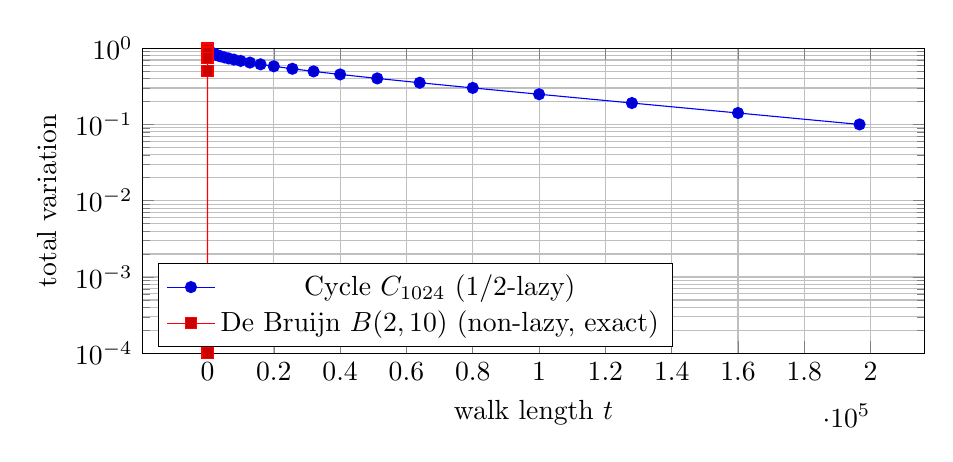
\begin{tikzpicture}
\begin{axis}[
  xmode=linear,
  width=0.95\linewidth,
  height=0.45\linewidth,
  xlabel={walk length $t$},
  ylabel={total variation},
  ymin=1e-4, ymax=1,
  ymode=log,
  legend style={at={(0.02,0.02)},anchor=south west},
  grid=both,
  unbounded coords=jump,
]
\addplot coordinates {
(1,0.997070)
(2,0.995117)
(3,0.993164)
(4,0.991211)
(5,0.989258)
(6,0.988770)
(8,0.986786)
(10,0.984949)
(12,0.983808)
(16,0.981296)
(20,0.979224)
(25,0.976890)
(32,0.974023)
(40,0.971308)
(50,0.968162)
(64,0.964399)
(80,0.960551)
(100,0.956326)
(128,0.951236)
(160,0.946076)
(200,0.940398)
(256,0.933467)
(320,0.926533)
(400,0.918901)
(512,0.909569)
(640,0.900256)
(800,0.890021)
(1000,0.878799)
(1280,0.865131)
(1600,0.851514)
(2000,0.836606)
(2560,0.818464)
(3200,0.800483)
(4000,0.780843)
(5120,0.757061)
(6400,0.733548)
(8000,0.707987)
(10000,0.680260)
(12800,0.646896)
(16000,0.614175)
(20000,0.578919)
(25600,0.536849)
(32000,0.495993)
(40000,0.452439)
(51200,0.401188)
(64000,0.352255)
(80000,0.301203)
(100000,0.248766)
(128000,0.190896)
(160000,0.141210)
(196657,0.100000)
};
\addlegendentry{Cycle $C_{1024}$ (1/2-lazy)}
\addplot coordinates {
(1,0.998047)
(2,0.996094)
(3,0.992188)
(4,0.984375)
(5,0.968750)
(6,0.937500)
(7,0.875000)
(8,0.750000)
(9,0.500000)
(10,1e-4)
(11,1e-4)
(12,1e-4)
};
\addlegendentry{De Bruijn $B(2,10)$ (non-lazy, exact)}
\end{axis}
\end{tikzpicture}
\caption{Smooth decay vs.\ finite-time cutoff in $\TV$. For log-$y$ display, exact zeros are clipped to $10^{-4}$.}
\label{fig:tv-cliff}
\end{figure}

\paragraph{Scaling check for the Chord ring+fingers overlay.}
Because the ring+fingers kernel is a circulant (Cayley) digraph on $\mathbb{Z}_n$,
the distribution and $\sigma=\max_{k\neq 0}|\lambda_k|$ can be computed exactly
by FFT. \cref{tab:chord-scale} reports $t_{0.1}$ and separation as $n=2^m$ grows.

\begin{table}[h]
\centering
\small
\setlength{\tabcolsep}{4pt}
\begin{tabular}{rrrrrrr}
\toprule
$n$ & $m$ & $\sigma$ & measured $t_{0.1}$ & TV@ $t_{0.1}$ & Sep@ $t_{0.1}$ & pred.\ $t_{0.1}$ \\
\midrule
256 & 8 & 0.875000 & 14 & 0.0963 & 0.7028 & 33 \\
512 & 9 & 0.888889 & 16 & 0.0978 & 0.7346 & 41 \\
1024 & 10 & 0.900000 & 18 & 0.0989 & 0.7633 & 49 \\
2048 & 11 & 0.909091 & 21 & 0.0876 & 0.7270 & 57 \\
\bottomrule
\end{tabular}
\caption{Chord ring+fingers scaling (1/2-lazy, start 0).}
\label{tab:chord-scale}
\end{table}



\paragraph{Sensitivity to compromise fraction: time-hidden first-hit.}
We sweep compromised fraction $\alpha$ and report (i) the probability of hitting
the compromised set within a horizon of 30 steps and (ii) leakage in a
\emph{time-hidden} model where the adversary learns only which compromised node
was hit first. (Construction details are in \cref{sec:reconstruct}.)

\begin{table}[h]
\centering
\small
\setlength{\tabcolsep}{3.5pt}
\begin{tabular}{r|rrr|rrr}
\toprule
 & \multicolumn{3}{c|}{Chord ring+fingers} & \multicolumn{3}{c}{Random 8-regular} \\
comp.\ frac & $P[\mathrm{hit}\le 30]$ & $I_{\mathrm{hid}}$ (bits) & MAP$_{\mathrm{hid}}$ &
$P[\mathrm{hit}\le 30]$ & $I_{\mathrm{hid}}$ (bits) & MAP$_{\mathrm{hid}}$ \\
\midrule
0.01 & 0.135986 & 0.046782 & 0.002159 & 0.118898 & 0.041077 & 0.002449 \\
0.05 & 0.526431 & 0.263719 & 0.007143 & 0.486559 & 0.237269 & 0.008565 \\
0.10 & 0.779561 & 0.587120 & 0.013865 & 0.742507 & 0.534519 & 0.017125 \\
0.20 & 0.958342 & 1.365357 & 0.029827 & 0.930654 & 1.236780 & 0.036783 \\
\bottomrule
\end{tabular}
\caption{Sanity-check ``first-hit'' sensitivity to compromised fraction ($n=1024$, horizon 30).}
\label{tab:firsthit-sweep}
\end{table}

\section{Reconstruction specification (compact)}\label{sec:reconstruct}
This section specifies enough to reconstruct \cref{tab:families,tab:firsthit-sweep}
from scratch. The goal is \emph{interoperable reimplementation}: an independent
implementation (human or LLM-generated) should reproduce values up to small
numerical tolerance.

\subsection{Graph families and kernels}
All kernels use \textbf{1/2-laziness}: with probability $1/2$ stay put; with
probability $1/2$ take a uniform random outgoing step.
All graphs are on $V=\{0,1,\dots,n-1\}$ with $n=1024$ unless stated.

\begin{itemize}[leftmargin=1.2em]
\item \textbf{Cycle $C_n$.} Undirected edges $(i,i\pm1\bmod n)$. Lazy walk as above.
\item \textbf{2D torus.} Grid $(\mathbb{Z}/32\mathbb{Z})^2$ mapped to $0..1023$;
neighbors differ by $\pm1$ in one coordinate (4-neighborhood); lazy walk.
\item \textbf{Hypercube $Q_{10}$.} Nodes are 10-bit strings; neighbors differ in
one bit (degree 10); lazy walk.
\item \textbf{Random 8-regular.} Sample an undirected 8-regular graph uniformly
at random (e.g., \texttt{networkx.random\_regular\_graph}) with RNG seed 0; lazy walk.
\item \textbf{Chord ring+fingers (directed).} Let $n=2^{10}$. From node $x$,
out-neighbors are $x+2^j\bmod n$ for $j=0,\dots,9$ (outdegree 10). Use the lazy
out-neighbor walk. (This digraph is regular and Eulerian, so $\pi$ is uniform.)
\item \textbf{Directed de Bruijn $B(2,10)$.} Nodes are length-10 bitstrings.
A move shifts left and appends a fresh random bit; use 1/2-laziness. (Uniform $\pi$.)
\end{itemize}

\subsection{Metrics and procedures}
\paragraph{Stationary distribution.}
For the regular families above, $\pi=\Unif(V)$. If implementing variants that
are not Eulerian, compute $\pi$ by power iteration until $\|\pi P-\pi\|_\infty$
is below $10^{-12}$.

\paragraph{TV and separation.}
Starting from the point mass at node 0, iterate $p_{t+1}=p_t P$.
Compute $\TV(p_t,\pi)=\tfrac12\sum_x|p_t(x)-\pi(x)|$ and
$\mathrm{sep}(p_t,\pi)=1-\min_x p_t(x)/\pi(x)$.

\paragraph{$t_{0.1}$.}
Define $t_{0.1}=\min\{t:\TV(p_t,\pi)\le 0.1\}$.

\paragraph{Singular value $\sigma$.}
Compute $\sigma=\sigma_2(\cD)$ where $\cD=\Pi^{1/2}P\Pi^{-1/2}$.
For uniform $\pi$, $\cD=P$. In sparse form, estimate the top singular values via
Lanczos/ARPACK SVD; report $\sigma_2$ to 6 decimals.

\paragraph{Predicted $t_{0.1}$.}
Solve for the smallest integer $t$ such that
$\tfrac12\sqrt{n}\,\sigma^{t}\le 0.1$ (using $\|v\|_1\le\sqrt{n}\|v\|_2$).

\subsection{First-hit time-hidden compromise sweep}
Fix horizon $H=30$ and compromised fraction $\alpha\in\{0.01,0.05,0.10,0.20\}$.
For each $\alpha$, sample a compromised set $C$ of size $\lfloor \alpha n\rfloor$
uniformly at random (seed 0). Sample $S\sim\Unif(V)$ and run a length-$H$ lazy
walk from $S$. Let $Y$ be the identity of the \emph{first} node in $C$ hit
(if any), else a special symbol $\bot$. In the \emph{time-hidden} model the
adversary observes $Y$.

Estimate:
\[
I_{\mathrm{hid}} = I(S;Y), \qquad
\mathrm{MAP}_{\mathrm{hid}} = \Prb[\hat S(Y)=S]\ \text{for the Bayes-optimal }\hat S.
\]
Use Monte Carlo with at least $10^5$ trials per $\alpha$ (the artifact uses more).
Treat results within $\pm 0.02$ bits (MI) and $\pm 2\times10^{-3}$ (MAP) as matching.

\paragraph{Sanity anchors.}
An implementation consistent with the above should reproduce
\cref{tab:families,tab:firsthit-sweep} within the stated tolerances.

\section{Conclusion}
Time reversal makes random-walk delegation anonymity explicit: the observed
delegate reveals a reversed walk. This yields sharp optimal distinguishability
and computable leakage certificates for directed overlays, and clarifies why
single-parameter spectral heuristics can fail on non-normal kernels. We provide
compact reconstruction guidance here to enable straightforward reimplementation.


\paragraph{Artifact availability.}
A full artifact bundle (scripts, full parameter sweeps, and raw outputs used to generate all tables and figures)
is intended to accompany this manuscript as supplementary material. To keep the main paper compact,
we include only a reconstruction specification and a small set of sanity-check tables; an independent
reimplementation should be straightforward from \cref{sec:reconstruct}.


\section*{References}
\begin{thebibliography}{99}\small

\bibitem{lpw}
D.~A. Levin, Y.~Peres, and E.~L. Wilmer.
\newblock \emph{Markov Chains and Mixing Times}, 2nd ed.
\newblock American Mathematical Society, 2017.

\bibitem{aldousdiaconis}
D.~Aldous and P.~Diaconis.
\newblock Strong stationary times and finite random walks.
\newblock \emph{Advances in Applied Mathematics}, 2(1):69--97, 1987.

\bibitem{fill}
J.~A. Fill.
\newblock The strength of weak convergence.
\newblock \emph{Stochastic Processes and their Applications}, 87(1):1--10, 2000.

\bibitem{reiterrubin}
M.~K. Reiter and A.~D. Rubin.
\newblock Crowds: Anonymity for {W}eb transactions.
\newblock \emph{ACM Transactions on Information and System Security}, 1(1):66--92, 1998.

\bibitem{backes}
M.~Backes, I.~Goldberg, A.~Kate, and T.~Toft.
\newblock Adding query privacy to robust {DHT}s.
\newblock In \emph{Proceedings of ASIACCS}, 2012.



\bibitem{shadowwalker}
P.~Mittal and N.~Borisov.
\newblock ShadowWalker: Peer-to-peer anonymous communication using redundant structured topologies.
\newblock In \emph{Proceedings of the 16th ACM Conference on Computer and Communications Security (CCS)}, 2009.

\bibitem{nisan}
A.~Panchenko, S.~Richter, and A.~Rache.
\newblock NISAN: Network information service for anonymization networks.
\newblock In \emph{Proceedings of the 16th ACM Conference on Computer and Communications Security (CCS)}, pages 141--150, 2009.

\bibitem{octopus}
Q.~Wang and N.~Borisov.
\newblock Octopus: A secure and anonymous DHT lookup.
\newblock In \emph{Proceedings of the 32nd IEEE International Conference on Distributed Computing Systems (ICDCS)}, pages 325--334, 2012.
\end{thebibliography}

\end{document}